\lecture{4}{3. September 2025}{ Control volume analysis II: Momentum \& energy equation}

\subsection{Momentum Equation for Inertial Control Volume}
We will now find a control volume form of Newton's second law. Note that in the following the coordinates (with respect to which velocities are meassured) are inertial, i.e. either at rest or moving at a constant speed with respect to an ``absolute'' set of coordinates.

We have previously defined Newton's second law for a system moving relative to an inertial coordinate system in \autoref{afs:N2} as:
\[ 
\textbf{F} = \frac{\mathrm{d}\textbf{P}}{\mathrm{d}t} \bigg)_{\mathrm{system}}
\]
where the linear momentum of the system is given by
\[ 
\textbf{P}_{\mathrm{system}} = \int_{M \left( \mathrm{system} \right)} \textbf{V} \, \mathrm{d}m = \int_{V (\mathrm{system})} \textbf{V} \rho \, \mathrm{d}V
\]
and the resultant force $\textbf{F}$ includes all surface and body forces acting on the system
\[ 
\textbf{F} = \textbf{F}_S + \textbf{F}_B
.\]

We have previously derived the relation between the system and control volume formulations in \autoref{eq:reytra} as:
\[ 
\frac{\mathrm{d}N}{\mathrm{d}t} \bigg)_{\mathrm{system}} = \frac{\partial }{\partial t} \int_{\mathrm{CV}} \eta \rho \, \mathrm{d}V + \int_{\mathrm{CS}} \eta \rho \textbf{V} \cdot \mathrm{d}\textbf{A}
.\]
In this we now set $N = \textbf{P}$ and $\eta = \textbf{V}$. We thus obtain:
\[ 
\frac{\mathrm{d}\textbf{P}}{\mathrm{d}t} \bigg)_{\mathrm{system}} = \frac{\partial }{\partial t} \int_{\mathrm{CV}} \textbf{V} \rho \, \mathrm{d}V + \int_{\mathrm{CS}} \textbf{V} \rho \textbf{V} \cdot \mathrm{d} \textbf{A}
.\]
Since in deriving \autoref{eq:reytra} the system and control volume conincided at $t_0$, then
\[ 
\textbf{F})_{\text{on system}} = \textbf{F})_{\text{on control volume}} = \textbf{F}_S + \textbf{F}_B
.\]
Now these can be combined as:
\begin{equation}\label{eq:convolN2}
  \textbf{F} = \textbf{F}_S + \textbf{F}_B = \frac{\partial}{\partial t} \int_{\mathrm{CV}} \textbf{V} \rho \, \mathrm{d}V + \int_{\mathrm{CS}} \textbf{V}\rho \textbf{V} \cdot \mathrm{d}\textbf{A} 
\end{equation}

For cases with uniform flow at each inlet and exit this becomes:
\[ 
\textbf{F} = \textbf{F}_S + \textbf{F}_B = \frac{\partial }{\partial t} \int_{\mathrm{CV}} \textbf{V} \rho \, \mathrm{d}V + \sum_{\mathrm{CS}} \textbf{V} \rho \textbf{V} \cdot \textbf{A}
.\]

When applying \autoref{eq:convolN2} we need to be a little careful. First we must choose a control volume and its control surface such that the volume integral and surface integral can be evaluated. In fluid mechanics the body force is usually gravity, so
\[ 
\textbf{F}_B = \int_{\mathrm{CV}} \rho \textbf{g} \, \mathrm{d}V = \textbf{W}_{\mathrm{CW}} = M \textbf{g}
.\]
In many applications the surface force is due to pressure,
\[ 
\textbf{F}_S = \int_A - p \, \mathrm{d}\textbf{A}
.\]

The momentum equation in \autoref{eq:convolN2} is a vector equation therefore it can be written in three scalar components as:
\begin{align*}
  F_x &= F_{S_x} + F_{B_x} = \frac{\partial }{\partial t} \int_{\mathrm{CV}} u \rho \, \mathrm{d}V + \int_{\mathrm{CS}} u \rho \textbf{V} \cdot \mathrm{d}\textbf{A} \\
    F_y &= F_{S_y} + F_{B_y} = \frac{\partial }{\partial t} \int_{\mathrm{CV}} v \rho \, \mathrm{d}V + \int_{\mathrm{CS}} v \rho \textbf{V} \cdot \mathrm{d}\textbf{A} \\
  F_z &= F_{S_z} + F_{B_z} = \frac{\partial }{\partial t} \int_{\mathrm{CV}} w \rho \, \mathrm{d}V + \int_{\mathrm{CS}} w \rho \textbf{V} \cdot \mathrm{d}\textbf{A}
.\end{align*}
Or in the case of uniform flow at each inlet and exit as
\begin{align*}
  F_x &= F_{S_x} + F_{B_x} = \frac{\partial }{\partial t}\int_{\mathrm{CV}} u \rho \, \mathrm{d}V + \sum_{\mathrm{CS}} u \rho \textbf{V} \cdot \textbf{A} \\
    F_y &= F_{S_y} + F_{B_y} = \frac{\partial }{\partial t}\int_{\mathrm{CV}} v \rho \, \mathrm{d}V + \sum_{\mathrm{CS}} v \rho \textbf{V} \cdot \textbf{A} \\
  F_z &= F_{S_z} + F_{B_z} = \frac{\partial }{\partial t}\int_{\mathrm{CV}} w \rho \, \mathrm{d}V + \sum_{\mathrm{CS}} w \rho \textbf{V} \cdot \textbf{A}
.\end{align*}

\subsubsection{Differential Control Volume Analysis}
The control volume approach that has been presented in the above is useful when applied to a finite region.

If we instead apply the approach to a differential control volume, we can obtain differential equations describing a flow field. Let us apply the continuity and momentum equations to a steady incompressible flow without friction as on \autoref{fig:f4_4}. The control volume is fixed in space and bounded by flow streamlines, and is thus an element of a stream tube. The length of the control volume is $\mathrm{d}s$. 

As the control volume is bounded by streamlines, flow across the boundaries of the control volume only happens at the end sections located at coordinates $s$ and $s + \mathrm{d}s$. Properties at the inlet sections are assigned arbitrary symbolic values and the properties at the outlet section are assumed to increase by differential amounts. 

\begin{figure} [ht]
  \centering
  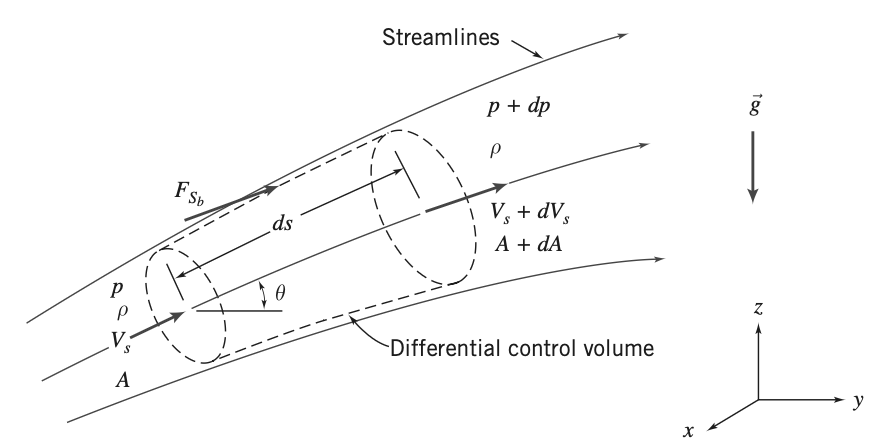
\includegraphics[width=0.5\linewidth]{./figures/f4_4.png}
  \caption{Differential control volume through a stream tube.}
  \label{fig:f4_4}
\end{figure}

Now we can apply the continuity equation,
\[ 
\frac{\partial }{\partial t} \int_{\mathrm{CV}} \rho \, \mathrm{d}V + \int_{\mathrm{CS}} \rho \textbf{V} \cdot \mathrm{d}\textbf{A} = 0
.\]
Which under assumptions of steady flow, no flow across the bounding streamlines and that the flow is incompressible ($\rho = \mathrm{constant}$), reduces to:
\[ 
\left( -\rho V_s A \right) + \left( \rho \left( V_s + \mathrm{d}V_s \right) \left( A + \mathrm{d}A \right) \right) = 0 \implies \rho \left( V_s + \mathrm{d}V_s \right) \left( A + \mathrm{d}A \right) = \rho V_s A
.\]
Simplifying we obtain
\[ 
V_s \, \mathrm{d}A + A \, \mathrm{d}V_s + \mathrm{d}A \, \mathrm{d}V_s = 0
.\]
The product of the differentials $\mathrm{d}A \, \mathrm{d}V_s \approx 0$ compared to the other terms so this can be neglected, leaving us with:
\[ 
V_s \, \mathrm{d}A + A \, \mathrm{d}V_s = 0
.\]

Using the streamwise component of the momentum equation we start with:
\[ 
F_{S_s} + F_{B_s} = \frac{\partial }{\partial t} \int_{\mathrm{CV}} u_s \rho \, \mathrm{d}V + \int_{\mathrm{CS}} u_s \rho \textbf{V} \cdot \mathrm{d}\textbf{A}
.\]
As we assume no friction $F_{S_s}$ is due to pressure forces only, and will thus have three terms:
\[ 
F_{S_s} = pA - \left( p + \mathrm{d}p \right)\left( A + \mathrm{d}A \right) + \left( p + \frac{\mathrm{d}p}{2} \right)\, \mathrm{d}A
.\]
The first and second terms in this are the pressure forces on the end faces of the control surface. The third term is $F_{s_b}$, the pressure force acting in the $s$ direction on the bounding stream surface. The above equation simplifies to
\[ 
F_{S_s} = - A \, \mathrm{d}p - \frac{1}{2} \, \mathrm{d}p \, \mathrm{d}A
.\]

The body force component in the $s$ direction is
\[ 
F_{B_s} = \rho g_s \, \mathrm{d}V = \rho \left( -g \sin \theta \right) \left( A + \frac{\mathrm{d}A}{2} \right)\, \mathrm{d}s
.\]
But $\sin \theta \, \mathrm{d}s = \mathrm{d}z$ so
\[ 
F_{B_s} = - \rho g \left( A + \frac{\mathrm{d}A}{2} \right)\, \mathrm{d}z
.\]
The momentum flux will be
\[ 
\int_{\mathrm{CS}} u_s \rho \textbf{V} \cdot \mathrm{d}\textbf{A} = V_s \left( - \rho V_s A \right) + \left( V_s + \mathrm{d}V_s \right) \left( \rho \left( V_s + \mathrm{d}V_s \right) \left( A + \mathrm{d}A \right) \right)
.\]
The two mass flux factors are equal from continuity so
\[ 
\int_{\mathrm{CS}} u_s \rho \textbf{V} \cdot \mathrm{d}\textbf{A} = V_s \left( - \rho V_s A \right) + \left( V_s + \mathrm{d}V_s \right) \left( \rho V_s A \right) = \rho V_s A \mathrm{d}V_s 
.\]
Substituting all of these into the momentum equation yields
\[ 
- A \, \mathrm{d}p - \frac{1}{2} \, \mathrm{d}p \, \mathrm{d}A - \rho g A \, \mathrm{d}z - \frac{1}{2} \rho g \, \mathrm{d}A \, \mathrm{d}z = \rho V_s A \mathrm{d}V_s
.\]
Dividing by $\rho A$ and noting that products of differentials are negligible we obtain:
\[ 
- \frac{\mathrm{d}p}{\rho} - g \, \mathrm{d}z = V_s \, \mathrm{d}V_s = d \left( \frac{V_s^2}{2} \right)
\]
or
\[ 
  \frac{\mathrm{d}p}{\rho} + d \left( \frac{V_s^2}{2} \right) + g \, \mathrm{d}z = 0
.\]
As the flow is incompressible and $\rho = \mathrm{constant}$ we can integrate this to obtain:
\[ 
\frac{p}{\rho} + \frac{V_s^2}{2} + gz = \mathrm{constant}
.\]
This is one form of the Bernoulli equation and it is only valid under the following restrictions:
\begin{enumerate}
  \item Steady flow
  \item No friction
  \item Flow along a streamline
  \item Incompressible flow
\end{enumerate}


\subsection{Momentum equation for Control Volume with Rectilinear Acceleration}
To develop the momentum equation for a linearly accelerating control volume, it is necessary to relate $\textbf{P}_{XYZ}$ to $\textbf{P}_{xyz}$. We begin by writing Newton's second law for a system, remembering the acceleration must be measured relative to an inertial reference frame that we have designated $XYZ$. We get
\[ 
\textbf{F} = \frac{\mathrm{d}\textbf{P}_{XYZ}}{\mathrm{d}t} \bigg)_{\mathrm{system}} = \frac{\mathrm{d}}{\mathrm{d}t} \int_{M (\mathrm{system})} \textbf{V}_{XYZ} \, \mathrm{d}m = \int_{M (\mathrm{system})} \frac{\mathrm{d}\textbf{V}_{XYZ}}{\mathrm{d}t} \, \mathrm{d}m
.\]
The velocities with respect to the inertial ($XYZ$) and the control volume coordinates ($xyz$) are related by the relative-motion equation:
\[ 
\textbf{V}_{XYZ} = \textbf{V}_{xyz} + \textbf{V}_{rf}
\]
where $\textbf{V}_{rf}$ is the velocity of the control volume coordinates $xyz$ with respect to the absolute $XYZ$. 

We assume the motion of $xyz$ is purely translational relative to the inertial reference frame $XYZ$, so:
\[ 
\frac{\mathrm{d}\textbf{V}_{XYZ}}{\mathrm{d}t} = \textbf{a}_{XYZ} = \frac{\mathrm{d}\textbf{V}_{xyz}}{\mathrm{d}t} + \frac{\mathrm{d}\textbf{V}_{rf}}{\mathrm{d}t} = \textbf{a}_{xyz} + \textbf{a}_{rf}
.\]
Substituting this into Newton's second law from above we get:
\[ 
\textbf{F} = \int_{M \left( \mathrm{system} \right)} \textbf{a}_{rf} \, \mathrm{d}m + \int_{M (\mathrm{system})} \frac{\mathrm{d}\textbf{V}_{xyz}}{\mathrm{d}t} \, \mathrm{d}m
\]
or
\[ 
\textbf{F} - \int_{M(\mathrm{system})} \textbf{a}_{rf} \, \mathrm{d}m = \frac{\mathrm{d}\textbf{P}_{xyz}}{\mathrm{d}t} \bigg)_{\mathrm{system}}
\]
where the linear momentum of the system is
\[ 
\textbf{P}_{xyz} )_{\mathrm{system}} = \int_{M (\mathrm{system})} \textbf{V}_{xyz} \, \mathrm{d}m = \int_{V (\mathrm{system})} \textbf{V}_{xyz} \rho \, \mathrm{d}V
\]
and the force $\textbf{F}$ includes all surface and body forces that are acting on the system.

To derive the control volume formulation of Newton's second law, we set $N = \textbf{P}_{xyz}$ and $\eta = \textbf{V}_{xyz}$. Substituting this into \autoref{eq:reytra} we obtain:
\[ 
\frac{\mathrm{d}\textbf{P}_{xyz}}{\mathrm{d}t} \bigg)_{\mathrm{system}} = \frac{\partial }{\partial t} \int_{\mathrm{CV}} \textbf{V}_{xyz} \rho \, \mathrm{d}V + \int_{\mathrm{CS}} \textbf{V}_{xyz} \rho \textbf{V}_{xyz} \cdot \mathrm{d}\textbf{A}
.\]
If we combine this with the linear momentum equation for the system we obtain:
\[ 
\textbf{F} - \int_{\mathrm{CV}} \textbf{a}_{rf} \rho \, \mathrm{d}V = \frac{\partial}{\partial t} \int_{\mathrm{CV}} \textbf{V}_{xyz} \rho \, \mathrm{d}V + \int_{\mathrm{CS}} \textbf{V}_{xyz} \rho \textbf{V}_{xyz} \cdot \mathrm{d}\textbf{A}
.\]
And since $\textbf{F} = \textbf{F}_S + \textbf{F}_B$ this becomes
\begin{equation}\label{eq:convolN2acc}
  \textbf{F}_S + \textbf{F}_B - \int_{\mathrm{CV}} \textbf{a}_{rf} \rho \, \mathrm{d}V = \frac{\partial}{\partial t} \int_{\mathrm{CV}} \textbf{V}_{xyz} \rho \, \mathrm{d}V + \int_{\mathrm{CS}} \textbf{V}_{xyz} \rho \textbf{V}_{xyz} \cdot \mathrm{d}\textbf{A}
\end{equation}
Comparing \autoref{eq:convolN2acc} to that for a non-accelerating control volume we see that they only differ by the introduction of the term $- \int_{\mathrm{CV}} \textbf{a}_{rf} \rho \, \mathrm{d}V$, and for a non-accelerating reference frame $\textbf{a}_{rf} = 0$ and it reduces to the equation for a non-accelerating reference frame. 

This can also be written in components as:
\begin{align*}
  F_{S_x} + F_{B_x} - \int_{\mathrm{CV}} a_{rf_x} \rho \, \mathrm{d}V &= \frac{\partial }{\partial t} \int_{\mathrm{CV}} u_{xyz} \rho \, \mathrm{d}V + \int_{\mathrm{CS}} u_{xyz} \rho \textbf{V}_{xyz} \cdot \mathrm{d}\textbf{A} \\
  F_{S_y} + F_{B_y} - \int_{\mathrm{CV}} a_{rf_y} \rho \, \mathrm{d}V &= \frac{\partial }{\partial t} \int_{\mathrm{CV}} v_{xyz} \rho \, \mathrm{d}V + \int_{\mathrm{CS}} v_{xyz} \rho \textbf{V}_{xyz} \cdot \mathrm{d}\textbf{A} \\
  F_{S_z} + F_{B_z} - \int_{\mathrm{CV}} a_{rf_z} \rho \, \mathrm{d}V &= \frac{\partial }{\partial t} \int_{\mathrm{CV}} w_{xyz} \rho \, \mathrm{d}V + \int_{\mathrm{CS}} w_{xyz} \rho \textbf{V}_{xyz} \cdot \mathrm{d}\textbf{A}
.\end{align*}

\subsection{The Angular-Momentum Principle}

\subsubsection{Equation for Fixed Control Volume}
The angular-momentum principle for a system in an inertial frame is
\[ 
\textbf{T} = \frac{\mathrm{d}\textbf{H}}{\mathrm{d}t} \bigg)_{\mathrm{system}}
\]
where $\textbf{T}$ is the total torque exerted on the system by its surroundings and $\textbf{H}$ is the angular momentum of the system.
\[ 
\textbf{H} = \int_{M (\mathrm{system})} \textbf{r} \times \textbf{V} \, \mathrm{d}m = \int_{V (\mathrm{system})} \textbf{r} \times \textbf{V} \rho \, \mathrm{d}V
.\]

If we let $\textbf{r}$ locate each mass or volume element of the system with respect to the coordinate system, then the torque $\textbf{T}$ applied to the system may be written:
\[ 
\textbf{T} = \textbf{r} \times \textbf{F}_s + \int_{M (\mathrm{system})} \textbf{r} \times \textbf{g} \, \mathrm{d}m + \textbf{T}_{\mathrm{shaft}}
.\]

The relation between the system and fixed control volume formulation is
\[ 
\frac{\mathrm{d}N}{\mathrm{d}t} \bigg)_{\mathrm{system}} = \frac{\partial }{\partial t} \int_{\mathrm{CV}} \eta \rho \, \mathrm{d}V + \int_{\mathrm{CS}} \eta \rho \textbf{V} \cdot \mathrm{d}\textbf{A}
.\]
where $N_{\mathrm{system}} = \int_{M (\mathrm{system})} \eta \, \mathrm{d}m$. If we set $N = \textbf{H}$ and $\eta = \textbf{r} \times \textbf{V}$ then:
\[ 
\frac{\mathrm{d}\textbf{H}}{\mathrm{d}t} \bigg)_{\mathrm{system}} = \frac{\partial }{\partial t} \int_{\mathrm{CV}} \textbf{r} \times \textbf{V} \rho \, \mathrm{d}V + \int_{\mathrm{CS}} \textbf{r} \times \textbf{V} \rho \textbf{V} \cdot \mathrm{d}\textbf{A}
.\]
Combining these we obtain:
\[ 
\textbf{r} \times \textbf{F}_s + \int_{M (\mathrm{system})} \textbf{r} \times \textbf{g} \, \mathrm{d}m + \textbf{T}_{\mathrm{shaft}} = \frac{\partial }{\partial t} \int_{\mathrm{CV}} \textbf{r} \times \textbf{V} \rho \, \mathrm{d}V + \int_{\mathrm{CS}} \textbf{r} \times \textbf{V} \rho \textbf{V} \cdot \mathrm{d}\textbf{A}
.\]
Since the system and control volume coincide at $t_0$ we have that $\textbf{T} = \textbf{T}_{\mathrm{CV}}$ and therefore:
\[ 
\textbf{r} \times \textbf{F}_s + \int_{\mathrm{CV}} \textbf{r} \times \textbf{g} \rho \, \mathrm{d}V + \textbf{T}_{\mathrm{shaft}} = \frac{\partial }{\partial t} \int_{\mathrm{CV}} \textbf{r} \times \textbf{V} \rho \, \mathrm{d}V + \int_{\mathrm{CS}} \textbf{r} \times \textbf{V} \rho \textbf{V} \cdot \mathrm{d}\textbf{A}
.\]

\subsection{The First Law of Thermodynamics}
We recall the system formulation of the first law of thermodynamics was
\[ 
\dot{Q} - \dot{W} = \frac{\mathrm{d}E}{\mathrm{d}t} \bigg)_{\mathrm{system}}
\]
where the total energy of the system is given by
\[ 
  E_{\mathrm{system}} = \int_{M (\mathrm{system})} e \, \mathrm{d}m = \int_{V (\mathrm{system})} e \rho \, \mathrm{d}V
\]
and
\[ 
e = u + \frac{V^2}{2} + gz
.\]
We set $N = E$ and $\eta = e$ in \autoref{eq:reytra} and obtain:
\[ 
\frac{\mathrm{d}E}{\mathrm{d}t} \bigg)_{\mathrm{system}} = \frac{\partial }{\partial t} \int_{\mathrm{CV}} e \rho \, \mathrm{d}V + \int_{\mathrm{CS}} e \rho \textbf{V} \cdot \mathrm{d} \textbf{A}
.\]
Since the system and control volume coincide at $t_0$ we have that $\left[ \dot{Q} - \dot{W} \right]_{\mathrm{system}} = \left[ \dot{Q} - \dot{W} \right]_{\text{control volume}}$. In light of this we get the control volume form of the first law of thermodynamics as:
\begin{equation} \label{eq:convolT1}
    \dot{Q} - \dot{W} = \frac{\partial }{\partial t} \int_{\mathrm{CV}} e \rho \, \mathrm{d}V + \int_{\mathrm{CS}} e \rho \textbf{V} \cdot \mathrm{d}\textbf{A}
\end{equation}
where
\[ 
e = u + \frac{V^2}{2} + gz
.\]
Note that for steady flow the right hand side of \autoref{eq:convolT1} is zero.

\subsubsection{Rate of Work Done by a Control Volume}
The rate of work done by a control volume is subdivided into four classifications,
\[ 
\dot{W} = \dot{W}_s + \dot{W}_{\mathrm{normal}} + \dot{W}_{\mathrm{shear}} + \dot{W}_{\mathrm{other}}
.\]

\paragraph{Shaft Work}
We will designate the shaft work $W_s$ and hence the rate of work transferred out through the control system by shaft work is designated $\dot{W}_s$.

\paragraph{Work Done by Normal Stresses at the Control Surface}
Work requires a force to act through a distance. Thus, when a force $\textbf{F}$ acts through an infinitesimal displacement $\mathrm{d}\textbf{s}$ the work done is given by
\[ 
\delta W = \textbf{F} \cdot \mathrm{d}\textbf{s}
.\]
If we divide this by the time increment $\Delta t$ and take the limit as $\Delta t \to 0$ we obtain the rate of work done by the force $\textbf{F}$ as:
\[ 
\dot{W} = \lim_{\Delta t \to 0} \frac{\delta W}{\Delta T} = \lim_{\Delta t \to 0}  \frac{\textbf{F} \cdot \mathrm{d}\textbf{s}}{\Delta t} \implies \dot{W} = \textbf{F} \cdot \textbf{V}
.\]
\begin{figure} [ht]
  \centering
  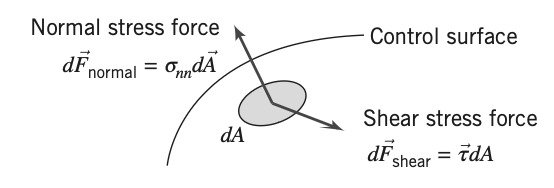
\includegraphics[width=0.5\linewidth]{./figures/f4_6.png}
  \caption{Normal and shear stress forces.}
  \label{fig:f4_6}
\end{figure}

We can use this to compute the rate of work done by normal and shear stresses. We consider the segment og control surface shown on \autoref{fig:f4_6}. For an element of area $\mathrm{d}\textbf{A}$ we can write an expression for the normal stress force $\mathrm{d}\textbf{F}_{\mathrm{normal}}$. This will be given by the normal stress $\sigma_{nn}$ multiplied by the vector element $\mathrm{d}\textbf{A}$. Hence:
\[ 
\mathrm{d}\textbf{F}_{\mathrm{normal}} \cdot \textbf{V} = \sigma_{nn} \, \mathrm{d}\textbf{A} \cdot \textbf{V}
.\]
Since the work out from the control volume is the negative work done on the control volume we get:
\[ 
\dot{W}_{\mathrm{normal}} = - \int_{\mathrm{CS}} \sigma_{nn} \, \mathrm{d}\textbf{A} \cdot \textbf{V} = -\int_{\mathrm{CS}} \sigma_{nn} \textbf{V} \cdot \mathrm{d}\textbf{A}
.\]

\paragraph{Work Done by Shear Stresses at the Control Surface}
As shown on \autoref{fig:f4_6} the shear force acting on an element of the control surface is given by:
\[ 
\mathrm{d} \textbf{F}_{\mathrm{shear}} = \bm{\tau} \, \mathrm{d}A
\]
where the shear stress vector, $\bm{\tau}$, is the shear stress acting in some direction in the plane of $\mathrm{d}A$. The rate of work done on the entire control surface by shear stresses is thus:
\[ 
\int_{\mathrm{CS}} \bm{\tau} \, \mathrm{d}A \cdot \textbf{V} = \int_{\mathrm{CS}} \bm{\tau} \cdot \textbf{V} \, \mathrm{d}A
.\]
Since the work out from the control volume is the negative of the work done on the control volume we get:
\[ 
\dot{W}_{\mathrm{shear}} = - \int_{\mathrm{CS}} \bm{\tau} \cdot \textbf{V} \, \mathrm{d}A
.\]
This is better expressed as three terms:
\[ 
  \dot{W}_{\mathrm{shear}} = - \int_{\mathrm{CS}} \bm{\tau} \cdot \textbf{V} \, \mathrm{d}A = - \int_{A (\mathrm{shafts})} \bm{\tau} \cdot \textbf{V} \, \mathrm{d}A - \int_{A (\text{solid surface})} \bm{\tau} \cdot \textbf{V} \, \mathrm{d}A - \int_{A (\mathrm{ports})} \bm{\tau} \cdot \textbf{V} \, \mathrm{d}A 
.\]
We have already accounted for the first term as $\dot{W}_s$ previously. At solid surfaces, $\textbf{V} = 0$, so the second term is zero (for a fixed control volume). Thus
\[ 
\dot{W}_{\mathrm{shear}} = - \int_{A (\mathrm{ports})} \bm{\tau} \cdot \textbf{V} \, \mathrm{d}A
.\]
For a control surface perpendicular to $\textbf{V}$ we get $\bm{\tau} \cdot \textbf{V} = 0$ and therefore $\dot{W}_{\mathrm{shear}} = 0$. 

\paragraph{Other Work}
This includes electrical and electromagnetic energy that could be absorbed by the control volume. This is absent in most cases, but for the general formulation it must be included.

With all terms in $\dot{W}$ evaluated, we get:
\[ 
\dot{W} = \dot{W}_s - \int_{\mathrm{CS}} \sigma_{nn} \textbf{V} \cdot \mathrm{d} \textbf{A} + \dot{W}_{\mathrm{shear}} + \dot{W}_{\mathrm{other}}
.\]
Substituting this into the original expression we get:
\[ 
\dot{Q} - \dot{W}_s + \int_{\mathrm{CS}} \sigma_{nn} \textbf{V} \cdot \mathrm{d}\textbf{A} - \dot{W}_{\mathrm{shear}} - \dot{W}_{other} = \frac{\partial }{\partial t} \int_{\mathrm{CV}} e \rho \, \mathrm{d}V + \int_{\mathrm{CS}} e \rho \textbf{V} \cdot \mathrm{d}\textbf{A}
.\]
Rearranging this and remembering $\rho = \frac{1}{v}$, where $v$ is specific volume we get:
\[ 
\dot{Q} - \dot{W}_s - \dot{W}_{\mathrm{shear}} - \dot{W}_{\mathrm{other}} = \frac{\partial }{\partial t}\int_{\mathrm{CV}} e \rho \, \mathrm{d}V + \int_{\mathrm{CS}} \left( e + \rho v \right)\rho \textbf{V} \cdot \mathrm{d}\textbf{A}
.\]
Substituting $e = u + \frac{V^2}{2} + gz$ into the last term we obtain the first law of thermodynamics for a control volume as:
\[ 
\dot{Q} - \dot{W}_s - \dot{W}_{\mathrm{shear}} - \dot{W}_{\mathrm{other}} = \frac{\partial }{\partial t} \int_{\mathrm{CV}} e \rho \, \mathrm{d}V + \int_{\mathrm{CS}} \left( u + p v + \frac{V^2}{2} + gz \right) \rho \textbf{V} \cdot \mathrm{d}\textbf{A}
.\]


\subsubsection{The Second Law of Thermodynamics}
The second law of thermodynamics applies to all fluid systems and is formulated as:
\[ 
\frac{\mathrm{d}S}{\mathrm{d}t} \bigg)_{\mathrm{system}} \geq \frac{1}{T} \dot{Q}
\]
where the total entropy of the system is given by
\[ 
S_{\mathrm{system}} = \int_{M (\mathrm{system})} s \, \mathrm{d}m = \int_{V (\mathrm{system})} s \rho \, \mathrm{d}V
.\]
We set $N = S$ and $\eta = s$ in \autoref{eq:reytra} and obtain
\[ 
\frac{\mathrm{d}S}{\mathrm{d}t} \bigg)_{\mathrm{system}} = \frac{\partial }{\partial t} \int_{\mathrm{CV}} s \rho \, \mathrm{d}V + \int_{\mathrm{CS}} s \rho \textbf{V} \cdot \mathrm{d}\textbf{A}
.\]
As the system and control volume coincide at $t_0$ we have that
\[ 
  \frac{1}{T} \dot{Q})_{\mathrm{system}} = \frac{1}{T}\dot{Q})_{\mathrm{CV}} = \int_{\mathrm{CS}} \frac{1}{T} \left( \frac{\dot{Q}}{A} \right) \, \mathrm{d}A 
.\]
Thus the control volume formulation of the second law of thermodynamics is:
\[ 
\frac{\partial }{\partial t} \int_{\mathrm{CV}} s \rho \, \mathrm{d}V + \int_{\mathrm{CS}} s \rho \textbf{V} \cdot \mathrm{d} \textbf{A} \geq \int_{\mathrm{CS}} \frac{1}{T} \left( \frac{\dot{Q}}{A} \right) \, \mathrm{d}A
.\]
Here the factor $\frac{\dot{Q}}{A}$ represents the heat flux per unit area into the control volume through the area element $\mathrm{d}A$. To evaluate the term
\[ 
\int_{\mathrm{CS}} \frac{1}{T} \left( \frac{\dot{Q}}{A} \right) \, \mathrm{d}A
.\]
both the local heat flux and local temperature $T$ must be known for each area element of the control surface.
